\documentclass{math}

\usepackage{tikz}

\title{University Physics 1A}
\author{Alvin Lin}
\date{November 6th, 2017}

\begin{document}

\maketitle

\section*{Torque Experiment}
\begin{center}
  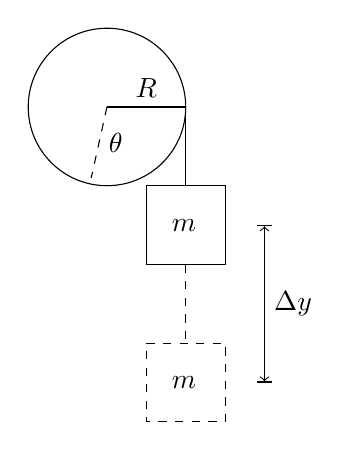
\begin{tikzpicture}
    \draw (0,0) circle (1cm);
    \draw (0,0) -- (1,0) node[pos=0.5,above] {\( R \)};
    \draw[dashed] (0,0) -- (-0.2,-0.9) node[pos=0.5,right] {\( \theta \)};
    \draw (1,0) -- (1,-1);
    \draw (0.5,-1) -- (1.5,-1) -- (1.5,-2) -- (0.5,-2) -- cycle
      node[pos=0.5,right,xshift=0.2cm] {\( m \)};
    \draw[dashed] (1,-2) -- (1,-3);
    \draw[dashed] (0.5,-3) -- (1.5,-3) -- (1.5,-4) -- (0.5,-4) -- cycle
      node[pos=0.5,right,xshift=0.2cm] {\( m \)};
    \draw[|<->|] (2,-1.5) -- (2,-3.5) node[pos=0.5,right] {\( \Delta y \)};
  \end{tikzpicture}
\end{center}
Find a formula for \( I \) in terms of \( \alpha \).
\begin{align*}
  \Delta y &= s = R\theta \quad F_{net} = ma \quad \tau_{net} = I\alpha \\
  -\frac{I\alpha}{R}-mg &= ma = mR\alpha \\
  -\frac{I\alpha}{R}-mR\alpha &= mg \\
  -\frac{I\alpha}{R} &= mg+mR\alpha \\
  I &= -\frac{R}{\alpha}(mg+mR\alpha) \\
  &= -\frac{mgR}{\alpha}-mR^2 \\
  &= -Rm(\frac{g}{\alpha}+R)
\end{align*}
\[ I = \frac{1}{2}M(R_1^2+R_2^2) \]

\begin{center}
  You can find all my notes at \url{http://omgimanerd.tech/notes}. If you have
  any questions, comments, or concerns, please contact me at
  alvin@omgimanerd.tech
\end{center}

\end{document}
